\subsection{Analog simulations}

All simulations of the analog circuitry were done using the AimSpice SPICE backend~\cite{AIMSpice} along with the AIMPlot~\cite{aimplot} frontend.

The camera was simulated as a whole with the spice code described in Appendix~\ref{ap:SpiceCode} listing~\ref{lst:cameratoplevel}.
In order to show that the camera is working as intended it was simulated with 750 pA current from the diodes and 2 ms exposure time as well as 50 pA diode current and 30 ms as shown in figure~\ref{fig:analog7502}~and~\ref{fig:analog5030}.
This shows that the camera can handle both maximum and minimum lighting conditions without over or under exposure.

A more typical situation is shown in figure~\ref{fig:analog4003} with 400 pA diode current and 4 ms exposure.

The camera is still possible to overexpose as shown in figure~\ref{fig:analog40010}, the user should therefore set the exposure to a sensible level.

\begin{figure}[H]
  \centering
  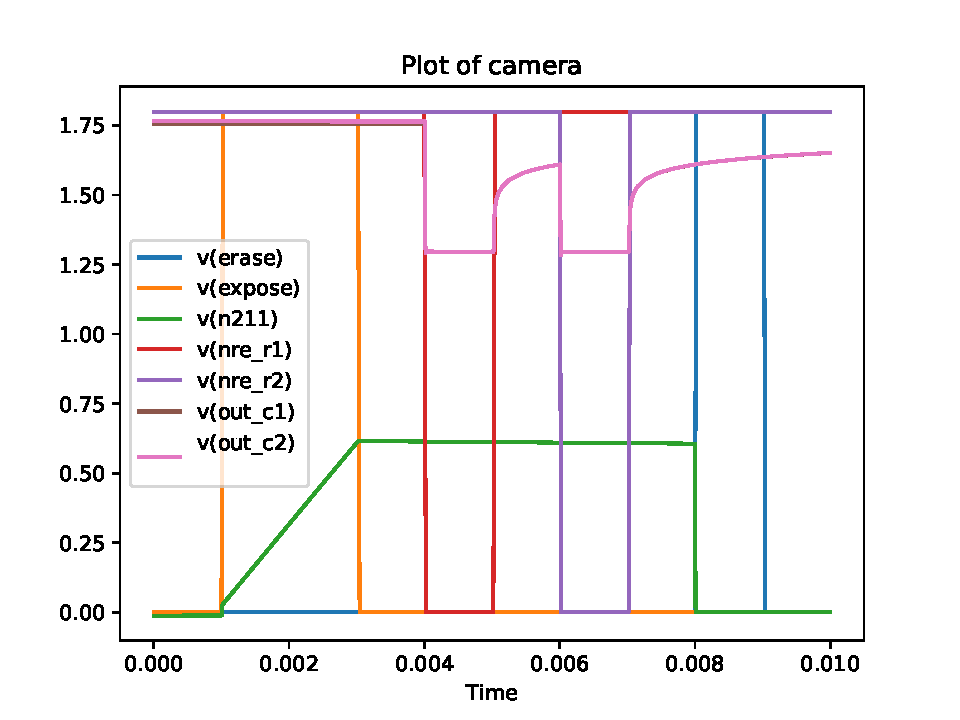
\includegraphics[width=0.75\textwidth]{../analog/camera7502}
  \caption{Analog camera tested with 750 pA and 2 ms}
  \label{fig:analog7502}
\end{figure}

\begin{figure}[H]
  \centering
  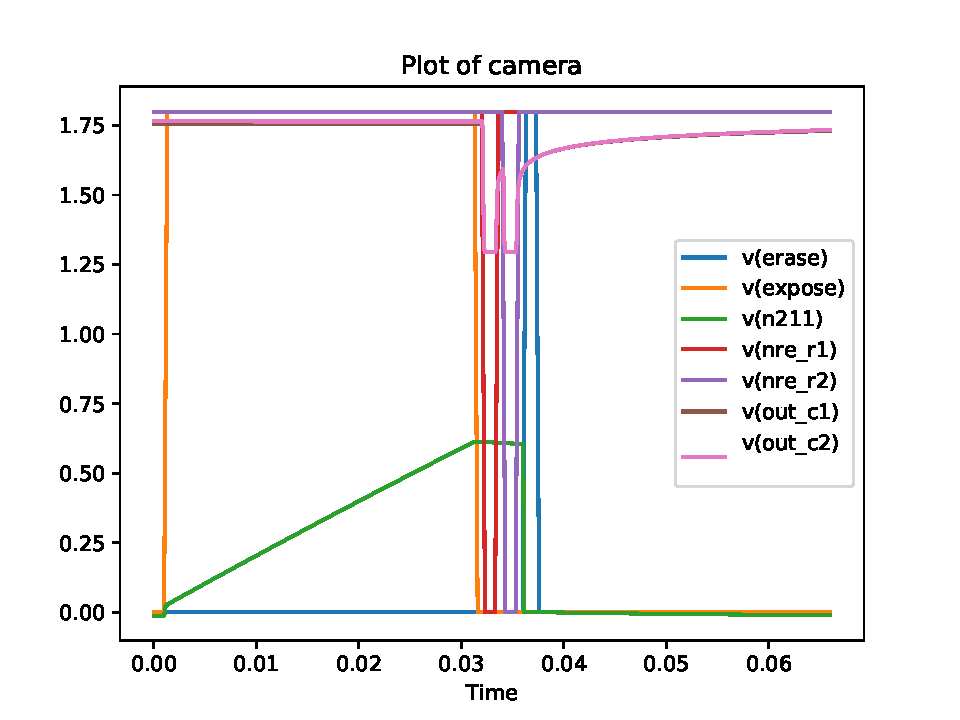
\includegraphics[width=0.75\textwidth]{../analog/camera5030}
  \caption{Analog camera tested with 50 pA and 30 ms}
  \label{fig:analog5030}
\end{figure}

\begin{figure}[H]
  \centering
  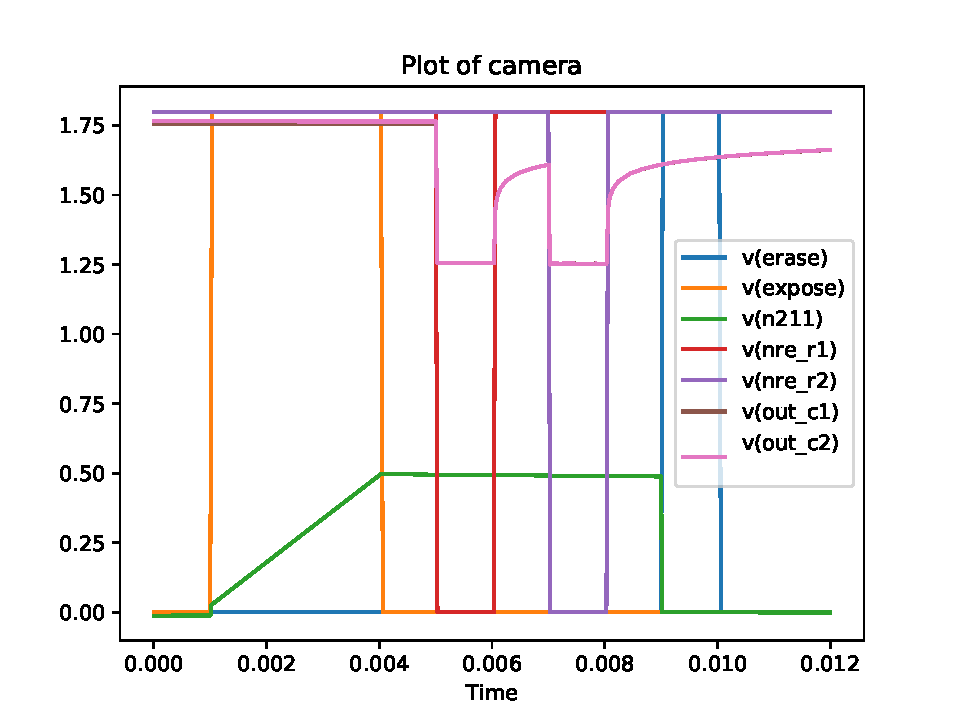
\includegraphics[width=0.75\textwidth]{../analog/camera4003typical}
  \caption{Analog camera tested with 400 pA and 3 ms}
  \label{fig:analog4003}
\end{figure}

\begin{figure}[H]
  \centering
  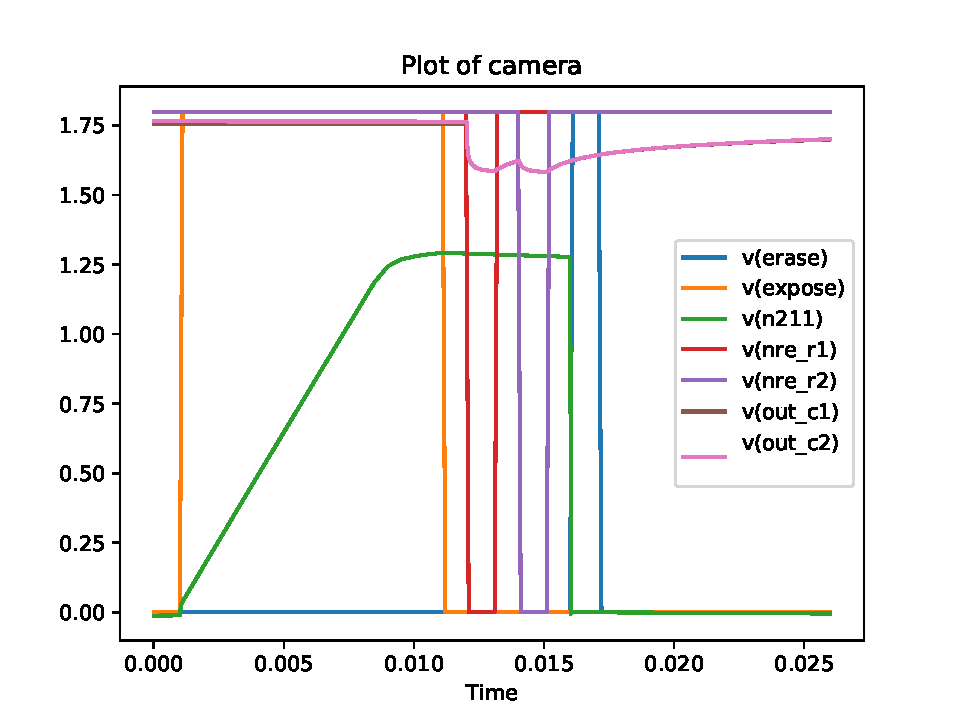
\includegraphics[width=0.75\textwidth]{../analog/camera40010overexposed}
  \caption{Analog camera tested with 400 pA and 10 ms}
  \label{fig:analog40010}
\end{figure}


Both the need for the current amplifiers and the possibility of leakage through M1 or M2 was discussed in Section~\ref{sec:AnalogDesign}.
In order to illustrate test these claims the camera was tested without the current amplifiers and with a leaky transistor M2 as shown in figures~\ref{fig:analog4003nocurrent}~and~\ref{fig:analogLeakingM2}.

\begin{figure}[H]
  \centering
  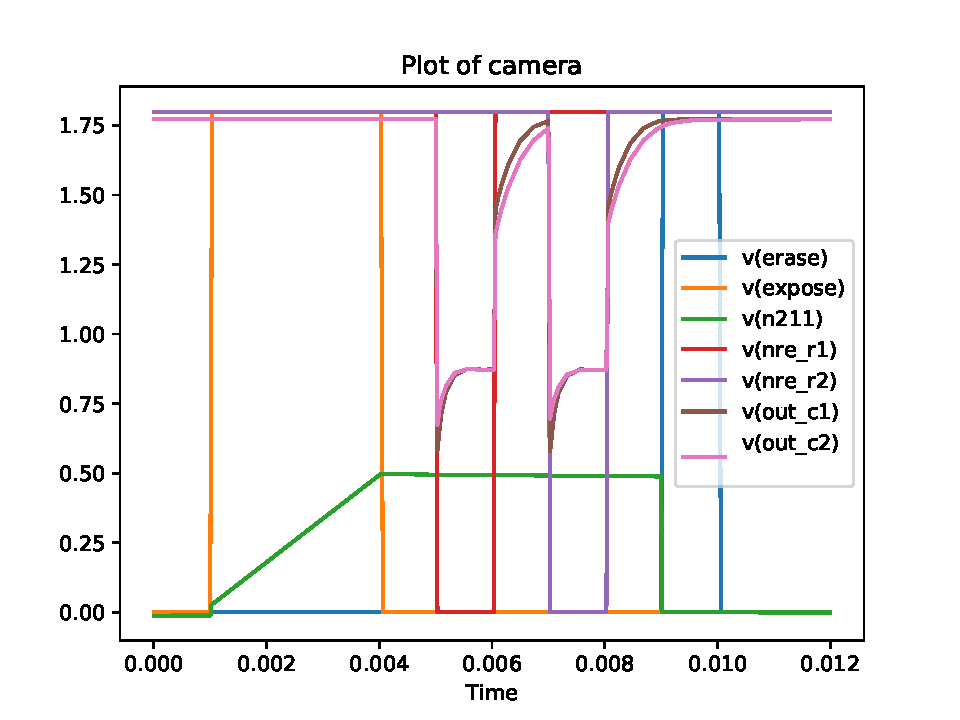
\includegraphics[width=0.75\textwidth]{../analog/camera4003nocurrentamp}
  \caption{Analog camera tested without current amplifiers}
  \label{fig:analog4003nocurrent}
\end{figure}

\begin{figure}[H]
  \centering
  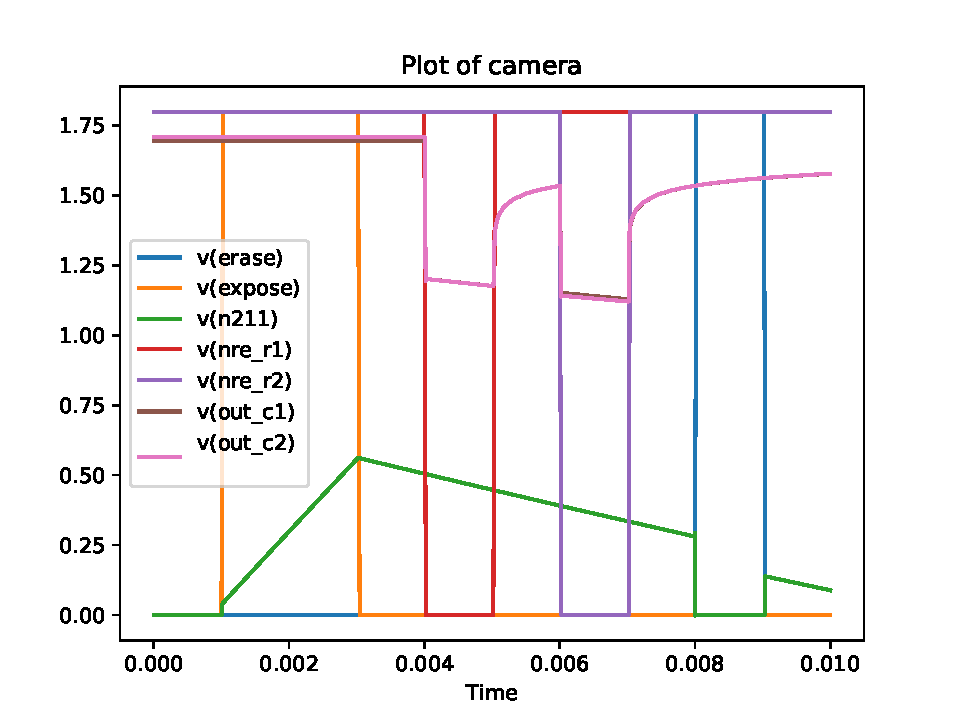
\includegraphics[width=0.75\textwidth]{../analog/cameraLeakingM2}
  \caption{Analog camera tested with transistor M2 tuned for maximum leakage}
  \label{fig:analogLeakingM2}
\end{figure}



\newpage
\subsection{Digital simulations}

Each individual module of the digital design was tested with test benches written in SystemVerilog as shown in Appendix~\ref{ap:VerilogCode}.
They were run using icarus-verilog~\cite{icarusVL} and the result visualized using GTKWave~\cite{gtkwave}.

Figure~\ref{fig:digexptest} shows the exposure counter, it demonstrates its minimum and maximum values of 2 and 30 being reached without bugs.

\begin{figure}[H]
  \centering
  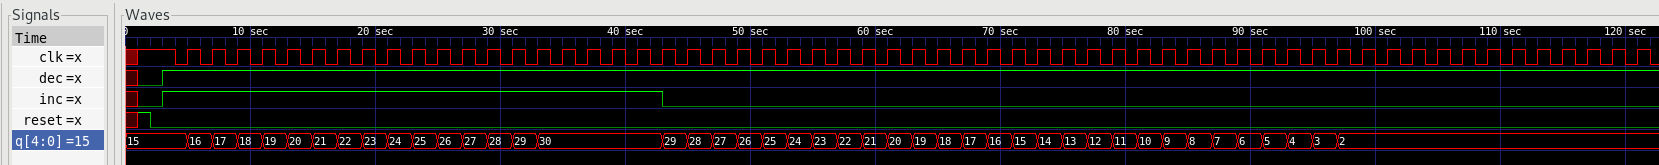
\includegraphics[width=\textwidth]{figures/expTest}
  \caption{Digital test of exposure time counter}
  \label{fig:digexptest}
\end{figure}

Figure~\ref{fig:digfcdtest} shows the countdown register for the exposure time. Its internal state \textit{data\_int} is shown in orange
to indicate that it is inaccessible from the outside, it is shown purely for informational purposes.\\
Note that the finished signal is triggered at $\text{\textit{data\_int}} \geq 1$ instead of $\text{\textit{data\_int}} \geq 0$,
this is in order to trigger the transition to the readout state on the same clock cycle that the register reaches 0.

\begin{figure}[H]
  \centering
  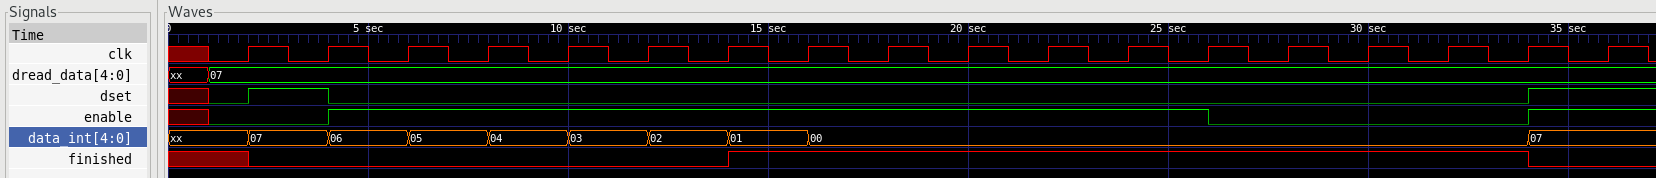
\includegraphics[width=\textwidth]{figures/fcdTest}
  \caption{Digital test of exposure countown circuit}
  \label{fig:digfcdtest}
\end{figure}

Figure~\ref{fig:digreadouttest} shows the readout sequencer, as with the countdown register the \textit{step} signal is shown in orange to indicate
that it is an internal inaccessible state.

\begin{figure}[H]
  \centering
  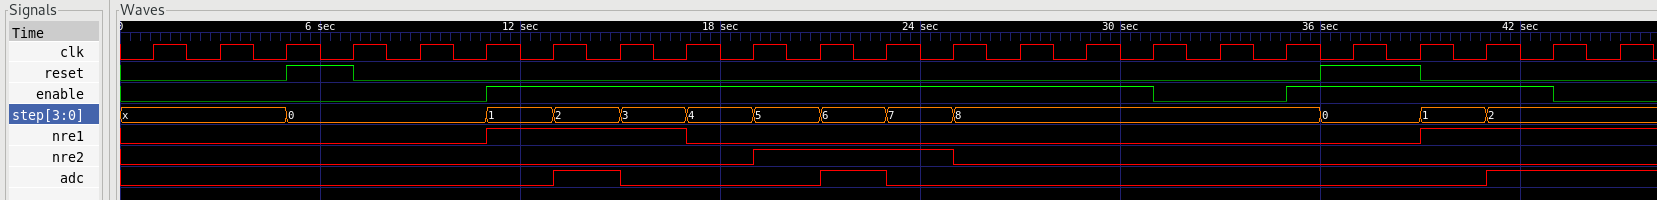
\includegraphics[width=\textwidth]{figures/readoutTest}
  \caption{Digital test of readout sequencer}
  \label{fig:digreadouttest}
\end{figure}


The camera control test-bench was to long to show on one page, its output is therefore split between figure~\ref{fig:digcamtest1}~and~\ref{fig:digcamtest2}.
Note that the orange signals does not indicate internal states, color is instead used purely for contrast between signals for easy reading.

\begin{figure}[H]
  \centering
  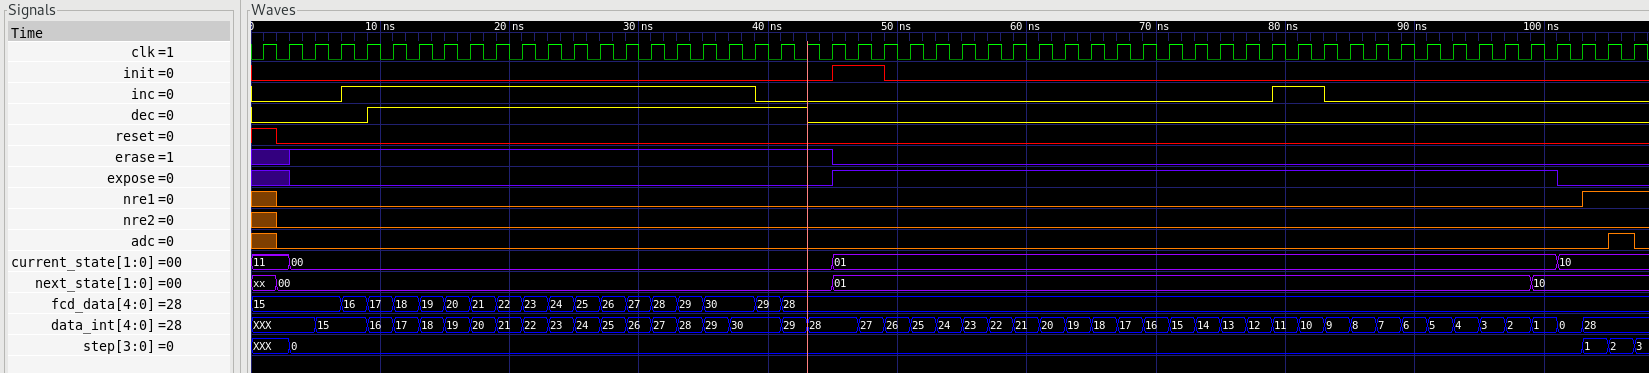
\includegraphics[width=\textwidth]{figures/cameraTest1}
  \caption{Digital test of the control circuitry part 1}
  \label{fig:digcamtest1}
\end{figure}

\begin{figure}[H]
  \centering
  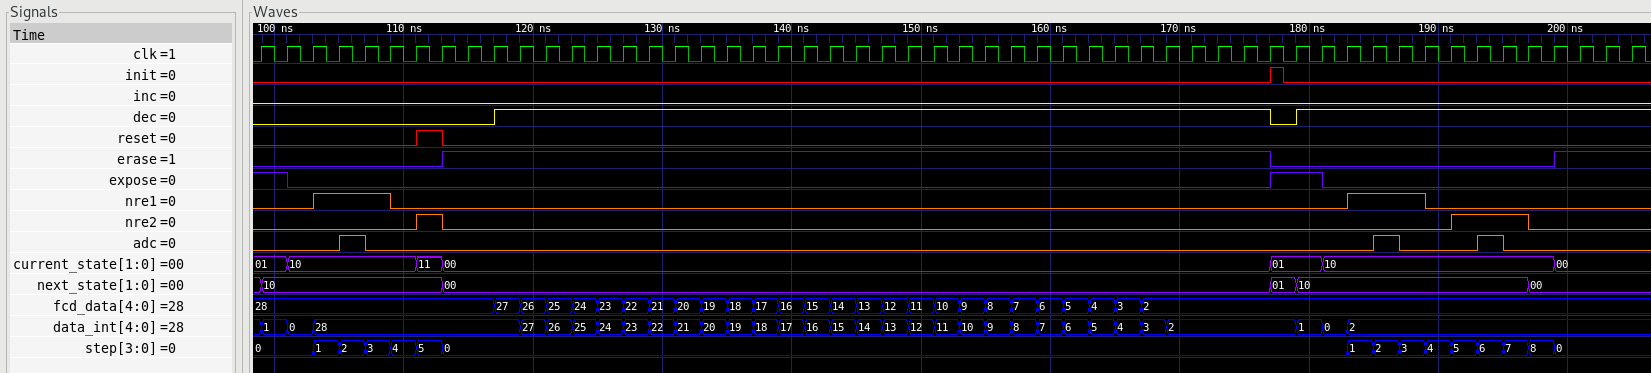
\includegraphics[width=\textwidth]{figures/cameraTest2}
  \caption{Digital test of the control circuitry part 2}
  \label{fig:digcamtest2}
\end{figure}